\documentclass[12pt,]{article}
\usepackage{lmodern}
\usepackage{amssymb,amsmath}
\usepackage{ifxetex,ifluatex}
\usepackage{fixltx2e} % provides \textsubscript
\ifnum 0\ifxetex 1\fi\ifluatex 1\fi=0 % if pdftex
  \usepackage[T1]{fontenc}
  \usepackage[utf8]{inputenc}
\else % if luatex or xelatex
  \ifxetex
    \usepackage{mathspec}
  \else
    \usepackage{fontspec}
  \fi
  \defaultfontfeatures{Ligatures=TeX,Scale=MatchLowercase}
    \setmainfont[]{Times New Roman}
\fi
% use upquote if available, for straight quotes in verbatim environments
\IfFileExists{upquote.sty}{\usepackage{upquote}}{}
% use microtype if available
\IfFileExists{microtype.sty}{%
\usepackage{microtype}
\UseMicrotypeSet[protrusion]{basicmath} % disable protrusion for tt fonts
}{}
\usepackage[margin=2.54cm]{geometry}
\usepackage{hyperref}
\hypersetup{unicode=true,
            pdftitle={Impacts of Land Use on Water Quality in Minnesota},
            pdfauthor={Keith Bollt, Jake Greif, Felipe Raby-Amadori, \& Lindsay Roth},
            pdfborder={0 0 0},
            breaklinks=true}
\urlstyle{same}  % don't use monospace font for urls
\usepackage{color}
\usepackage{fancyvrb}
\newcommand{\VerbBar}{|}
\newcommand{\VERB}{\Verb[commandchars=\\\{\}]}
\DefineVerbatimEnvironment{Highlighting}{Verbatim}{commandchars=\\\{\}}
% Add ',fontsize=\small' for more characters per line
\usepackage{framed}
\definecolor{shadecolor}{RGB}{248,248,248}
\newenvironment{Shaded}{\begin{snugshade}}{\end{snugshade}}
\newcommand{\AlertTok}[1]{\textcolor[rgb]{0.94,0.16,0.16}{#1}}
\newcommand{\AnnotationTok}[1]{\textcolor[rgb]{0.56,0.35,0.01}{\textbf{\textit{#1}}}}
\newcommand{\AttributeTok}[1]{\textcolor[rgb]{0.77,0.63,0.00}{#1}}
\newcommand{\BaseNTok}[1]{\textcolor[rgb]{0.00,0.00,0.81}{#1}}
\newcommand{\BuiltInTok}[1]{#1}
\newcommand{\CharTok}[1]{\textcolor[rgb]{0.31,0.60,0.02}{#1}}
\newcommand{\CommentTok}[1]{\textcolor[rgb]{0.56,0.35,0.01}{\textit{#1}}}
\newcommand{\CommentVarTok}[1]{\textcolor[rgb]{0.56,0.35,0.01}{\textbf{\textit{#1}}}}
\newcommand{\ConstantTok}[1]{\textcolor[rgb]{0.00,0.00,0.00}{#1}}
\newcommand{\ControlFlowTok}[1]{\textcolor[rgb]{0.13,0.29,0.53}{\textbf{#1}}}
\newcommand{\DataTypeTok}[1]{\textcolor[rgb]{0.13,0.29,0.53}{#1}}
\newcommand{\DecValTok}[1]{\textcolor[rgb]{0.00,0.00,0.81}{#1}}
\newcommand{\DocumentationTok}[1]{\textcolor[rgb]{0.56,0.35,0.01}{\textbf{\textit{#1}}}}
\newcommand{\ErrorTok}[1]{\textcolor[rgb]{0.64,0.00,0.00}{\textbf{#1}}}
\newcommand{\ExtensionTok}[1]{#1}
\newcommand{\FloatTok}[1]{\textcolor[rgb]{0.00,0.00,0.81}{#1}}
\newcommand{\FunctionTok}[1]{\textcolor[rgb]{0.00,0.00,0.00}{#1}}
\newcommand{\ImportTok}[1]{#1}
\newcommand{\InformationTok}[1]{\textcolor[rgb]{0.56,0.35,0.01}{\textbf{\textit{#1}}}}
\newcommand{\KeywordTok}[1]{\textcolor[rgb]{0.13,0.29,0.53}{\textbf{#1}}}
\newcommand{\NormalTok}[1]{#1}
\newcommand{\OperatorTok}[1]{\textcolor[rgb]{0.81,0.36,0.00}{\textbf{#1}}}
\newcommand{\OtherTok}[1]{\textcolor[rgb]{0.56,0.35,0.01}{#1}}
\newcommand{\PreprocessorTok}[1]{\textcolor[rgb]{0.56,0.35,0.01}{\textit{#1}}}
\newcommand{\RegionMarkerTok}[1]{#1}
\newcommand{\SpecialCharTok}[1]{\textcolor[rgb]{0.00,0.00,0.00}{#1}}
\newcommand{\SpecialStringTok}[1]{\textcolor[rgb]{0.31,0.60,0.02}{#1}}
\newcommand{\StringTok}[1]{\textcolor[rgb]{0.31,0.60,0.02}{#1}}
\newcommand{\VariableTok}[1]{\textcolor[rgb]{0.00,0.00,0.00}{#1}}
\newcommand{\VerbatimStringTok}[1]{\textcolor[rgb]{0.31,0.60,0.02}{#1}}
\newcommand{\WarningTok}[1]{\textcolor[rgb]{0.56,0.35,0.01}{\textbf{\textit{#1}}}}
\usepackage{longtable,booktabs}
\usepackage{graphicx,grffile}
\makeatletter
\def\maxwidth{\ifdim\Gin@nat@width>\linewidth\linewidth\else\Gin@nat@width\fi}
\def\maxheight{\ifdim\Gin@nat@height>\textheight\textheight\else\Gin@nat@height\fi}
\makeatother
% Scale images if necessary, so that they will not overflow the page
% margins by default, and it is still possible to overwrite the defaults
% using explicit options in \includegraphics[width, height, ...]{}
\setkeys{Gin}{width=\maxwidth,height=\maxheight,keepaspectratio}
\IfFileExists{parskip.sty}{%
\usepackage{parskip}
}{% else
\setlength{\parindent}{0pt}
\setlength{\parskip}{6pt plus 2pt minus 1pt}
}
\setlength{\emergencystretch}{3em}  % prevent overfull lines
\providecommand{\tightlist}{%
  \setlength{\itemsep}{0pt}\setlength{\parskip}{0pt}}
\setcounter{secnumdepth}{5}
% Redefines (sub)paragraphs to behave more like sections
\ifx\paragraph\undefined\else
\let\oldparagraph\paragraph
\renewcommand{\paragraph}[1]{\oldparagraph{#1}\mbox{}}
\fi
\ifx\subparagraph\undefined\else
\let\oldsubparagraph\subparagraph
\renewcommand{\subparagraph}[1]{\oldsubparagraph{#1}\mbox{}}
\fi

%%% Use protect on footnotes to avoid problems with footnotes in titles
\let\rmarkdownfootnote\footnote%
\def\footnote{\protect\rmarkdownfootnote}

%%% Change title format to be more compact
\usepackage{titling}

% Create subtitle command for use in maketitle
\providecommand{\subtitle}[1]{
  \posttitle{
    \begin{center}\large#1\end{center}
    }
}

\setlength{\droptitle}{-2em}

  \title{Impacts of Land Use on Water Quality in Minnesota}
    \pretitle{\vspace{\droptitle}\centering\huge}
  \posttitle{\par}
  \subtitle{\url{https://github.com/lhr12/HDA_Project}}
  \author{Keith Bollt, Jake Greif, Felipe Raby-Amadori, \& Lindsay Roth}
    \preauthor{\centering\large\emph}
  \postauthor{\par}
    \date{}
    \predate{}\postdate{}
  

\begin{document}
\maketitle
\begin{abstract}
Abstract tbd
\end{abstract}

\newpage
\tableofcontents 
\newpage
\listoftables 
\newpage
\listoffigures 
\newpage

\hypertarget{research-question-and-rationale}{%
\section{Research Question and
Rationale}\label{research-question-and-rationale}}

\begin{itemize}
\tightlist
\item
  Land use has a large impact on nutrient runoff into streams, lakes,
  and other water bodies
\item
  Minnesota has wide variety of land uses. Inlcudes large urban centers,
  natural lands, and agricultural area.
\item
  Nutrient management has been a challenge for states in the effort to
  control harmful algal blooms and coastal dead zones.
\item
  Understanding the causes of nutrient problems will better inform
  management strategies.
\end{itemize}

Research questions:

\begin{enumerate}
\def\labelenumi{\arabic{enumi}.}
\item
  What are the predictors of nutrients based on land use in watersheds
  in the state of Minnesota?
\item
  How do you characterize seasonal variation between the predictors of
  nutrients?
\end{enumerate}

Goals: * Determine how land use, watershed size, and ecoregion explain
variation in nutrient loading indicators. * Discern whether there a
seasonal trends in nutrient loading indicators based on land use types,
watershed size, and ecoregion. * Provide insight to inform decisions
about nutrient managment practices based on land use types, watershed
size, and ecoregion.

\newpage

\hypertarget{dataset-information}{%
\section{Dataset Information}\label{dataset-information}}

The data used in this analysis include data from the Lake Multi-Scaled
Geospatial and Temporal Database (LAGOSNE) and the EPA ecoregion spatial
datasets.

LAGOSNE is a collection of several data modules that contain information
on lakes in the northern United States. The modules contain data from
thousands of lakes in 17 states in the northeastern and midwestern
United States, from Missouri to Maine. The dataset includes a complete
list of all lakes bigger than 4 hectacres in the 17 state area, and
water quality data on a large number of lakes, spanning every state.

Ecoregions are used by planning managers to understand the type of land
use that occurs in different regions of the United States. There are
different levels of ecoregions. Level 1 divides North America into 15
ecological regions, while Level IV offers fine ecological resolution for
each state. This data was published by the U.S. EPA Office of Research
and Development (ORD) - National Health and Environmental Effects
Research Laboratory (NHEERL). For the purposes of our project, we
selected Level III ecoregions because in our judgement, Level IV
ecoregions are more specific than the type of analysis we are performing
calls for.

\begin{longtable}[]{@{}llll@{}}
\toprule
ï..Column.Name & Description & Units & Variable.Type\tabularnewline
\midrule
\endhead
chla & Chlorophyll a & mg/L & Depedent\tabularnewline
secchi & Secchi depth & m & Depedent\tabularnewline
Urban.pct & Percent urban land cover & \% & Independent-
fixed\tabularnewline
Undeveloped.pct & Percent natural land cover & \% & Independent-
fixed\tabularnewline
Ag.pct & Percent agricultural land cover & \% & Independent-
fixed\tabularnewline
LakeIWS.Ratio & Lake surface area to watershed area ratio & N/A &
Independent- fixed\tabularnewline
Season & Early, prime, and late growing ``seasons'' & N/A & Independent-
fixed\tabularnewline
US\_L3NAME & Level 3 ecoregions & N/A & Independent-
random\tabularnewline
\bottomrule
\end{longtable}

\newpage

\hypertarget{exploratory-data-analysis-and-wrangling}{%
\section{Exploratory Data Analysis and
Wrangling}\label{exploratory-data-analysis-and-wrangling}}

\begin{Shaded}
\begin{Highlighting}[]
\CommentTok{#load LAGOS data}
\NormalTok{LAGOSdata <-}\StringTok{ }\KeywordTok{lagosne_load}\NormalTok{()}
\end{Highlighting}
\end{Shaded}

\begin{verbatim}
## Warning in `_f`(version = version, fpath = fpath): LAGOSNE version
## unspecified, loading version: 1.087.3
\end{verbatim}

\begin{Shaded}
\begin{Highlighting}[]
\CommentTok{# creating specific lagos files}
\NormalTok{LAGOSstate <-}\StringTok{ }\NormalTok{LAGOSdata}\OperatorTok{$}\NormalTok{state}
\NormalTok{LAGOSlocus <-}\StringTok{ }\NormalTok{LAGOSdata}\OperatorTok{$}\NormalTok{locus}
\NormalTok{LAGOSnutrient <-}\StringTok{ }\NormalTok{LAGOSdata}\OperatorTok{$}\NormalTok{epi_nutr}
\NormalTok{LAGOSiwslulc <-}\StringTok{ }\NormalTok{LAGOSdata}\OperatorTok{$}\NormalTok{iws.lulc}
\NormalTok{LAGOSiws <-}\StringTok{ }\NormalTok{LAGOSdata}\OperatorTok{$}\NormalTok{iws}
\end{Highlighting}
\end{Shaded}

\begin{Shaded}
\begin{Highlighting}[]
\CommentTok{#State 14: Minnesota}
\NormalTok{LAGOSlocus.MN <-}\StringTok{ }\NormalTok{LAGOSlocus }\OperatorTok\StringTok{ }\KeywordTok{filter}\NormalTok{ (state_zoneid }\OperatorTok{==}\StringTok{ "State_14"}\NormalTok{)}
\NormalTok{LAGOSnutrient.MN <-}\StringTok{ }\NormalTok{LAGOSlocus.MN }\OperatorTok
\StringTok{  }\KeywordTok{left_join}\NormalTok{(LAGOSnutrient, }\DataTypeTok{by =} \StringTok{"lagoslakeid"}\NormalTok{) }
\end{Highlighting}
\end{Shaded}

\begin{Shaded}
\begin{Highlighting}[]
\CommentTok{#getting the area of the iws}
\NormalTok{LAGOSiws.area <-}\StringTok{ }\KeywordTok{select}\NormalTok{(LAGOSiws, }\StringTok{"lagoslakeid"}\NormalTok{, }\StringTok{"iws_ha"}\NormalTok{)}

\CommentTok{#joining MN locus with iwslulc and adding the area of IWS}
\NormalTok{LAGOSiws.MN <-}\StringTok{ }\NormalTok{LAGOSlocus.MN }\OperatorTok\StringTok{ }
\StringTok{  }\KeywordTok{left_join}\NormalTok{(LAGOSiwslulc, }\DataTypeTok{by =} \StringTok{"lagoslakeid"}\NormalTok{) }\OperatorTok
\StringTok{  }\KeywordTok{left_join}\NormalTok{(LAGOSiws.area, }\DataTypeTok{by =} \StringTok{"lagoslakeid"}\NormalTok{)}

\CommentTok{##selecting 2011 lulc}
\NormalTok{LAGOSiws2011.MN <-}\StringTok{ }\NormalTok{LAGOSiws.MN }\OperatorTok\StringTok{ }
\StringTok{  }\KeywordTok{select}\NormalTok{(lagoslakeid,state_zoneid, lake_area_ha, iws_ha,}
\NormalTok{         iws_nlcd2011_pct_}\DecValTok{11}\NormalTok{, iws_nlcd2011_pct_}\DecValTok{21}\NormalTok{, iws_nlcd2011_pct_}\DecValTok{22}\NormalTok{,}
\NormalTok{         iws_nlcd2011_pct_}\DecValTok{23}\NormalTok{, iws_nlcd2011_pct_}\DecValTok{24}\NormalTok{, iws_nlcd2011_pct_}\DecValTok{31}\NormalTok{,}
\NormalTok{         iws_nlcd2011_pct_}\DecValTok{41}\NormalTok{, iws_nlcd2011_pct_}\DecValTok{42}\NormalTok{, iws_nlcd2011_pct_}\DecValTok{43}\NormalTok{,}
\NormalTok{         iws_nlcd2011_pct_}\DecValTok{52}\NormalTok{, iws_nlcd2011_pct_}\DecValTok{71}\NormalTok{, iws_nlcd2011_pct_}\DecValTok{81}\NormalTok{,}
\NormalTok{         iws_nlcd2011_pct_}\DecValTok{82}\NormalTok{, iws_nlcd2011_pct_}\DecValTok{90}\NormalTok{, iws_nlcd2011_pct_}\DecValTok{95}\NormalTok{)}
\end{Highlighting}
\end{Shaded}

\begin{Shaded}
\begin{Highlighting}[]
\CommentTok{#filtering state nutrient data #FRA. We can expand this range}
\NormalTok{LAGOSnutrient.MN.skinny <-}\StringTok{ }\NormalTok{LAGOSnutrient.MN }\OperatorTok
\StringTok{  }\KeywordTok{filter}\NormalTok{(sampledate }\OperatorTok{>}\StringTok{ "2008-12-31"} \OperatorTok{&}\StringTok{ }\NormalTok{sampledate }\OperatorTok{<}\StringTok{ "2015-01-01"}\NormalTok{)}
\end{Highlighting}
\end{Shaded}

\begin{Shaded}
\begin{Highlighting}[]
\CommentTok{##Joining iws.lulc and nutrient}
\NormalTok{LAGOSiws.nutrient.}\FloatTok{2011.}\NormalTok{MN <-}\StringTok{  }\KeywordTok{left_join}\NormalTok{(LAGOSnutrient.MN.skinny,}
\NormalTok{                                        LAGOSiws2011.MN, }\DataTypeTok{by =}
                                          \KeywordTok{c}\NormalTok{(}\StringTok{"lagoslakeid"}\NormalTok{, }\StringTok{"lake_area_ha"}\NormalTok{)) }

\NormalTok{LAGOSiws.nutrient.}\FloatTok{2011.}\NormalTok{MN <-}\StringTok{ }\NormalTok{LAGOSiws.nutrient.}\FloatTok{2011.}\NormalTok{MN }\OperatorTok
\StringTok{  }\KeywordTok{select}\NormalTok{(lagoslakeid, nhd_lat, nhd_long, lake_area_ha, lake_perim_meters,}
\NormalTok{         iws_zoneid, iws_ha, state_zoneid.x, elevation_m, sampledate, chla,secchi, }
\NormalTok{         iws_nlcd2011_pct_}\DecValTok{11}\NormalTok{, iws_nlcd2011_pct_}\DecValTok{21}\NormalTok{, iws_nlcd2011_pct_}\DecValTok{22}\NormalTok{, }
\NormalTok{         iws_nlcd2011_pct_}\DecValTok{23}\NormalTok{, iws_nlcd2011_pct_}\DecValTok{24}\NormalTok{, iws_nlcd2011_pct_}\DecValTok{31}\NormalTok{, }
\NormalTok{         iws_nlcd2011_pct_}\DecValTok{41}\NormalTok{, iws_nlcd2011_pct_}\DecValTok{42}\NormalTok{, iws_nlcd2011_pct_}\DecValTok{43}\NormalTok{, }
\NormalTok{         iws_nlcd2011_pct_}\DecValTok{52}\NormalTok{, iws_nlcd2011_pct_}\DecValTok{71}\NormalTok{, iws_nlcd2011_pct_}\DecValTok{81}\NormalTok{, }
\NormalTok{         iws_nlcd2011_pct_}\DecValTok{82}\NormalTok{, iws_nlcd2011_pct_}\DecValTok{90}\NormalTok{, iws_nlcd2011_pct_}\DecValTok{95}\NormalTok{)}
\end{Highlighting}
\end{Shaded}

Visualizing the Secchi and Chla data.

\begin{Shaded}
\begin{Highlighting}[]
\KeywordTok{ggplot}\NormalTok{(LAGOSiws.nutrient.}\FloatTok{2011.}\NormalTok{MN, }
       \KeywordTok{aes}\NormalTok{(}\DataTypeTok{x =}\NormalTok{ sampledate, }\DataTypeTok{y =}\NormalTok{ secchi, }\DataTypeTok{color =}\NormalTok{ lagoslakeid)) }\OperatorTok{+}
\StringTok{  }\KeywordTok{scale_color_viridis_c}\NormalTok{(}\DataTypeTok{option =} \StringTok{"plasma"}\NormalTok{) }\OperatorTok{+}
\StringTok{  }\KeywordTok{geom_line}\NormalTok{() }
\end{Highlighting}
\end{Shaded}

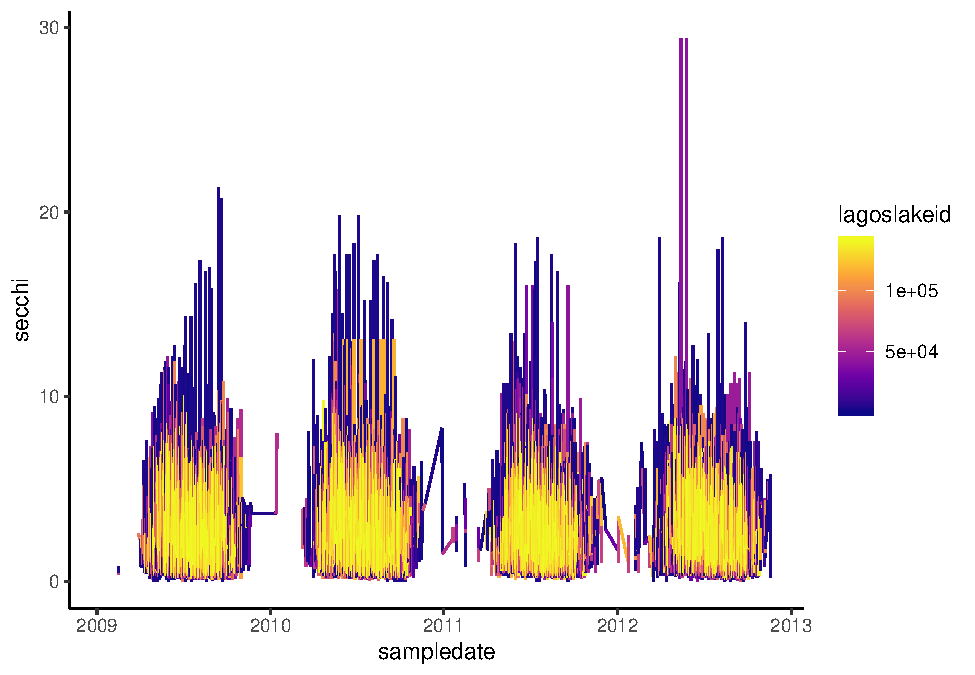
\includegraphics{Bollt_Greif_Raby_Roth_Project_Draft_files/figure-latex/Visualize_data-1.pdf}

\begin{Shaded}
\begin{Highlighting}[]
\KeywordTok{ggplot}\NormalTok{(LAGOSiws.nutrient.}\FloatTok{2011.}\NormalTok{MN, }
       \KeywordTok{aes}\NormalTok{(}\DataTypeTok{x =}\NormalTok{ sampledate, }\DataTypeTok{y =}\NormalTok{ chla, }\DataTypeTok{color =}\NormalTok{ lagoslakeid)) }\OperatorTok{+}
\StringTok{  }\KeywordTok{scale_color_viridis_c}\NormalTok{(}\DataTypeTok{option =} \StringTok{"plasma"}\NormalTok{) }\OperatorTok{+}
\StringTok{  }\KeywordTok{geom_line}\NormalTok{() }
\end{Highlighting}
\end{Shaded}

\begin{verbatim}
## Warning: Removed 10 rows containing missing values (geom_path).
\end{verbatim}

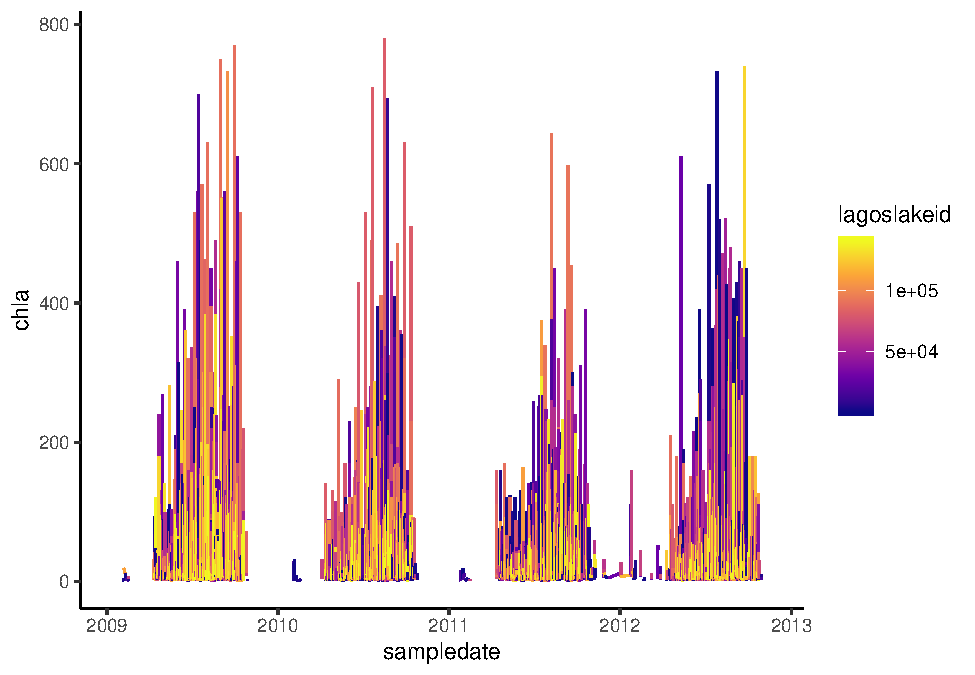
\includegraphics{Bollt_Greif_Raby_Roth_Project_Draft_files/figure-latex/Visualize_data-2.pdf}

Creating full data frame.

\begin{Shaded}
\begin{Highlighting}[]
\NormalTok{LAGOS.MN.processed <-}\StringTok{ }\NormalTok{LAGOSiws.nutrient.}\FloatTok{2011.}\NormalTok{MN }\OperatorTok
\StringTok{  }\KeywordTok{mutate}\NormalTok{(}\DataTypeTok{Water.pct =}\NormalTok{ iws_nlcd2011_pct_}\DecValTok{11}\NormalTok{,}
         \DataTypeTok{Urban.pct =}\NormalTok{ iws_nlcd2011_pct_}\DecValTok{21} \OperatorTok{+}\StringTok{ }\NormalTok{iws_nlcd2011_pct_}\DecValTok{22} \OperatorTok{+}
\StringTok{           }\NormalTok{iws_nlcd2011_pct_}\DecValTok{23} \OperatorTok{+}\StringTok{ }\NormalTok{iws_nlcd2011_pct_}\DecValTok{24}\NormalTok{,}
         \DataTypeTok{Undeveloped.pct =}\NormalTok{ iws_nlcd2011_pct_}\DecValTok{31} \OperatorTok{+}\StringTok{ }\NormalTok{iws_nlcd2011_pct_}\DecValTok{41} \OperatorTok{+}
\StringTok{           }\NormalTok{iws_nlcd2011_pct_}\DecValTok{42} \OperatorTok{+}\StringTok{ }\NormalTok{iws_nlcd2011_pct_}\DecValTok{43} \OperatorTok{+}\StringTok{ }
\StringTok{           }\NormalTok{iws_nlcd2011_pct_}\DecValTok{52} \OperatorTok{+}\StringTok{ }\NormalTok{iws_nlcd2011_pct_}\DecValTok{90} \OperatorTok{+}\StringTok{ }\NormalTok{iws_nlcd2011_pct_}\DecValTok{95}\NormalTok{,}
         \DataTypeTok{Ag.pct =}\NormalTok{  iws_nlcd2011_pct_}\DecValTok{81} \OperatorTok{+}\StringTok{ }\NormalTok{iws_nlcd2011_pct_}\DecValTok{82} \OperatorTok{+}\StringTok{ }
\StringTok{           }\NormalTok{iws_nlcd2011_pct_}\DecValTok{71}\NormalTok{) }\OperatorTok
\StringTok{  }\KeywordTok{select}\NormalTok{(}\OperatorTok{-}\KeywordTok{c}\NormalTok{(iws_nlcd2011_pct_}\DecValTok{11}\NormalTok{, iws_nlcd2011_pct_}\DecValTok{21}\NormalTok{, iws_nlcd2011_pct_}\DecValTok{22}\NormalTok{, }
\NormalTok{            iws_nlcd2011_pct_}\DecValTok{23}\NormalTok{, iws_nlcd2011_pct_}\DecValTok{24}\NormalTok{, iws_nlcd2011_pct_}\DecValTok{31}\NormalTok{, }
\NormalTok{            iws_nlcd2011_pct_}\DecValTok{41}\NormalTok{, iws_nlcd2011_pct_}\DecValTok{42}\NormalTok{, iws_nlcd2011_pct_}\DecValTok{43}\NormalTok{, }
\NormalTok{            iws_nlcd2011_pct_}\DecValTok{52}\NormalTok{, iws_nlcd2011_pct_}\DecValTok{71}\NormalTok{, iws_nlcd2011_pct_}\DecValTok{81}\NormalTok{, }
\NormalTok{            iws_nlcd2011_pct_}\DecValTok{82}\NormalTok{, iws_nlcd2011_pct_}\DecValTok{90}\NormalTok{, iws_nlcd2011_pct_}\DecValTok{95}\NormalTok{)) }\OperatorTok
\StringTok{  }\KeywordTok{na.omit}\NormalTok{() }\OperatorTok
\StringTok{  }\KeywordTok{mutate}\NormalTok{(}\DataTypeTok{LakeIWS.Ratio =}\NormalTok{ lake_area_ha}\OperatorTok{/}\NormalTok{iws_ha) }\OperatorTok
\StringTok{  }\KeywordTok{mutate}\NormalTok{(}\DataTypeTok{DOY =} \KeywordTok{yday}\NormalTok{(sampledate))}
\end{Highlighting}
\end{Shaded}

\begin{Shaded}
\begin{Highlighting}[]
\CommentTok{#We are creating growing seasons; early, prime, late. }
\CommentTok{#They will be based off of water temperature and day of year. }
\CommentTok{#We choose May 15 and October 1 because these are arbitrary but }
\CommentTok{#approximate bookends to the prime growing season.}

\NormalTok{LAGOS.MN.processed}\OperatorTok{$}\NormalTok{EarlyTrue <-}\StringTok{ }
\StringTok{  }\NormalTok{LAGOS.MN.processed}\OperatorTok{$}\NormalTok{DOY }\OperatorTok{<}\StringTok{ }\DecValTok{136} \CommentTok{#Before May 15}
\NormalTok{LAGOS.MN.processed}\OperatorTok{$}\NormalTok{PrimeTrue <-}\StringTok{ }
\StringTok{  }\NormalTok{LAGOS.MN.processed}\OperatorTok{$}\NormalTok{DOY }\OperatorTok{>=}\DecValTok{136} \OperatorTok{&}\StringTok{ }\NormalTok{LAGOS.MN.processed}\OperatorTok{$}\NormalTok{DOY }\OperatorTok{<=}\StringTok{ }\DecValTok{273} \CommentTok{#May 15 to September 30}
\NormalTok{LAGOS.MN.processed}\OperatorTok{$}\NormalTok{LateTrue <-}\StringTok{ }
\StringTok{  }\NormalTok{LAGOS.MN.processed}\OperatorTok{$}\NormalTok{DOY }\OperatorTok{>}\StringTok{ }\DecValTok{273}  \CommentTok{#October 1 and later}

\NormalTok{LAGOS.MN.processed}\OperatorTok{$}\NormalTok{EarlyTrue <-}\StringTok{ }
\StringTok{  }\KeywordTok{ifelse}\NormalTok{(LAGOS.MN.processed}\OperatorTok{$}\NormalTok{EarlyTrue }\OperatorTok{==}\StringTok{ }\OtherTok{TRUE}\NormalTok{, }\StringTok{"Early"}\NormalTok{, }\StringTok{"No"}\NormalTok{)}
\NormalTok{LAGOS.MN.processed}\OperatorTok{$}\NormalTok{PrimeTrue <-}\StringTok{ }
\StringTok{  }\KeywordTok{ifelse}\NormalTok{(LAGOS.MN.processed}\OperatorTok{$}\NormalTok{PrimeTrue }\OperatorTok{==}\StringTok{ }\OtherTok{TRUE}\NormalTok{, }\StringTok{"Prime"}\NormalTok{, }\StringTok{"No"}\NormalTok{)}
\NormalTok{LAGOS.MN.processed}\OperatorTok{$}\NormalTok{LateTrue <-}\StringTok{ }
\StringTok{  }\KeywordTok{ifelse}\NormalTok{(LAGOS.MN.processed}\OperatorTok{$}\NormalTok{LateTrue }\OperatorTok{==}\StringTok{ }\OtherTok{TRUE}\NormalTok{, }\StringTok{"Late"}\NormalTok{, }\StringTok{"No"}\NormalTok{)}

\NormalTok{LAGOS.MN.processed}\OperatorTok{$}\NormalTok{Season <-}\StringTok{ }\NormalTok{LAGOS.MN.processed}\OperatorTok{$}\NormalTok{EarlyTrue }\OperatorTok{==}\StringTok{ "Early"}
  
\NormalTok{LAGOS.MN.processed}\OperatorTok{$}\NormalTok{Season[LAGOS.MN.processed}\OperatorTok{$}\NormalTok{EarlyTrue }\OperatorTok{==}\StringTok{ "Early"}\NormalTok{] <-}\StringTok{ "Early"}
\NormalTok{LAGOS.MN.processed}\OperatorTok{$}\NormalTok{Season[LAGOS.MN.processed}\OperatorTok{$}\NormalTok{PrimeTrue }\OperatorTok{==}\StringTok{ "Prime"}\NormalTok{] <-}\StringTok{ "Prime"}
\NormalTok{LAGOS.MN.processed}\OperatorTok{$}\NormalTok{Season[LAGOS.MN.processed}\OperatorTok{$}\NormalTok{LateTrue }\OperatorTok{==}\StringTok{ "Late"}\NormalTok{] <-}\StringTok{ "Late"}

\NormalTok{LAGOS.MN.processed  <-}\StringTok{ }\NormalTok{LAGOS.MN.processed }\OperatorTok
\StringTok{  }\KeywordTok{select}\NormalTok{(}\OperatorTok{-}\KeywordTok{c}\NormalTok{(EarlyTrue, PrimeTrue, LateTrue))}
\end{Highlighting}
\end{Shaded}

\begin{Shaded}
\begin{Highlighting}[]
\NormalTok{LAGOS.MN.processed.sf <-}\StringTok{ }\KeywordTok{st_as_sf}\NormalTok{(LAGOS.MN.processed, }
                                  \DataTypeTok{coords =} \KeywordTok{c}\NormalTok{(}\StringTok{"nhd_long"}\NormalTok{, }\StringTok{"nhd_lat"}\NormalTok{), }\DataTypeTok{crs =} \DecValTok{4326}\NormalTok{)}

\NormalTok{LAGOS.MN.processed.UTM.sf <-}\StringTok{ }\KeywordTok{st_transform}\NormalTok{(LAGOS.MN.processed.sf, }\DataTypeTok{crs=}\DecValTok{26917}\NormalTok{)}

\NormalTok{MN.Ecoregions.sf <-}\StringTok{ }\KeywordTok{st_read}\NormalTok{(}\StringTok{'./Data/Raw/mn_eco_l3.shp'}\NormalTok{)}
\end{Highlighting}
\end{Shaded}

\begin{verbatim}
## Reading layer `mn_eco_l3' from data source `C:\Users\Felipe\OneDrive - Duke University\1. DUKE\Ramos 3 Semestre\722 Hydro Data\HDA_Project_FRA\data\raw\mn_eco_l3.shp' using driver `ESRI Shapefile'
## Simple feature collection with 7 features and 13 fields
## geometry type:  MULTIPOLYGON
## dimension:      XY
## bbox:           xmin: -91854.57 ymin: 2278542 xmax: 489296.4 ymax: 2930681
## epsg (SRID):    NA
## proj4string:    +proj=aea +lat_1=29.5 +lat_2=45.5 +lat_0=23 +lon_0=-96 +x_0=0 +y_0=0 +datum=NAD83 +units=m +no_defs
\end{verbatim}

\begin{Shaded}
\begin{Highlighting}[]
\CommentTok{#Selecting level 3 ecoregions names}
\NormalTok{MN.Ecoregions.sf <-}\StringTok{ }\KeywordTok{select}\NormalTok{(MN.Ecoregions.sf, US_L3NAME)}

\NormalTok{MN.Ecoregions.UTM.sf <-}\StringTok{ }\KeywordTok{st_transform}\NormalTok{(MN.Ecoregions.sf, }\DataTypeTok{crs=}\DecValTok{26917}\NormalTok{)}

\NormalTok{LAGOS.MN.processed.sf <-}\StringTok{ }\KeywordTok{st_join}\NormalTok{(LAGOS.MN.processed.UTM.sf, MN.Ecoregions.UTM.sf)}
\end{Highlighting}
\end{Shaded}

\begin{Shaded}
\begin{Highlighting}[]
\CommentTok{#Creating sf seasons files}
\NormalTok{LAGOS.MN.processed.Early.sf <-}\StringTok{ }\KeywordTok{filter}\NormalTok{(LAGOS.MN.processed.sf, Season }\OperatorTok{==}\StringTok{ "Early"}\NormalTok{)}
\NormalTok{LAGOS.MN.processed.Prime.sf <-}\StringTok{ }\KeywordTok{filter}\NormalTok{(LAGOS.MN.processed.sf, Season }\OperatorTok{==}\StringTok{ "Prime"}\NormalTok{)}
\NormalTok{LAGOS.MN.processed.Late.sf <-}\StringTok{ }\KeywordTok{filter}\NormalTok{(LAGOS.MN.processed.sf, Season }\OperatorTok{==}\StringTok{ "Late"}\NormalTok{)}

\CommentTok{#Creating regular season files (doesn't have ecoregions column)}
\NormalTok{LAGOS.MN.processed.Early <-}\StringTok{ }\KeywordTok{filter}\NormalTok{(LAGOS.MN.processed, Season }\OperatorTok{==}\StringTok{ "Early"}\NormalTok{)}
\NormalTok{LAGOS.MN.processed.Prime <-}\StringTok{ }\KeywordTok{filter}\NormalTok{(LAGOS.MN.processed, Season }\OperatorTok{==}\StringTok{ "Prime"}\NormalTok{)}
\NormalTok{LAGOS.MN.processed.Late <-}\StringTok{ }\KeywordTok{filter}\NormalTok{(LAGOS.MN.processed, Season }\OperatorTok{==}\StringTok{ "Late"}\NormalTok{)}
\end{Highlighting}
\end{Shaded}

Visualizing preliminary trends with scatterplots.

\begin{Shaded}
\begin{Highlighting}[]
\KeywordTok{ggplot}\NormalTok{(LAGOS.MN.processed.Late.sf, }\KeywordTok{aes}\NormalTok{(}\DataTypeTok{x =}\NormalTok{ Undeveloped.pct, }\DataTypeTok{y =}\NormalTok{ secchi)) }\OperatorTok{+}
\KeywordTok{geom_point}\NormalTok{() }\OperatorTok{+}
\KeywordTok{geom_smooth}\NormalTok{(}\DataTypeTok{method=}\NormalTok{lm) }\OperatorTok{+}
\KeywordTok{xlab}\NormalTok{(}\KeywordTok{expression}\NormalTok{(}\StringTok{"Undeveloped %"}\NormalTok{)) }\OperatorTok{+}
\KeywordTok{ylab}\NormalTok{(}\KeywordTok{expression}\NormalTok{(}\StringTok{"Secchi Depth (m)"}\NormalTok{)) }\OperatorTok{+}
\KeywordTok{ggtitle}\NormalTok{(}\StringTok{"Undeveloped % vs Secchi Depth Scatterplot, Late Season"}\NormalTok{) }\OperatorTok{+}
\KeywordTok{theme}\NormalTok{(}\DataTypeTok{plot.title =} \KeywordTok{element_text}\NormalTok{(}\DataTypeTok{hjust =} \FloatTok{0.5}\NormalTok{))}
\end{Highlighting}
\end{Shaded}

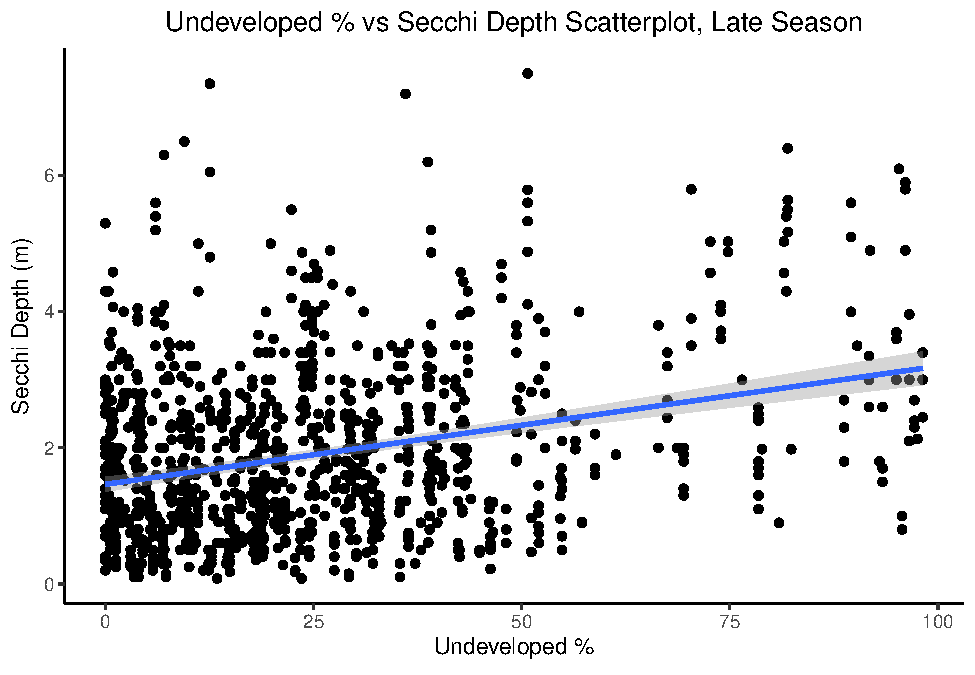
\includegraphics{Bollt_Greif_Raby_Roth_Project_Draft_files/figure-latex/scatterplots-1.pdf}

\begin{Shaded}
\begin{Highlighting}[]
\KeywordTok{ggplot}\NormalTok{(LAGOS.MN.processed.Late.sf, }\KeywordTok{aes}\NormalTok{(}\DataTypeTok{x =}\NormalTok{ Urban.pct, }\DataTypeTok{y =}\NormalTok{ secchi)) }\OperatorTok{+}
\KeywordTok{geom_point}\NormalTok{() }\OperatorTok{+}
\KeywordTok{geom_smooth}\NormalTok{(}\DataTypeTok{method=}\NormalTok{lm) }\OperatorTok{+}
\KeywordTok{xlab}\NormalTok{(}\KeywordTok{expression}\NormalTok{(}\StringTok{"Urban %"}\NormalTok{)) }\OperatorTok{+}
\KeywordTok{ylab}\NormalTok{(}\KeywordTok{expression}\NormalTok{(}\StringTok{"Secchi Depth (m)"}\NormalTok{)) }\OperatorTok{+}
\KeywordTok{ggtitle}\NormalTok{(}\StringTok{"Urban % vs Secchi Depth Scatterplot, Late Season"}\NormalTok{) }\OperatorTok{+}
\KeywordTok{theme}\NormalTok{(}\DataTypeTok{plot.title =} \KeywordTok{element_text}\NormalTok{(}\DataTypeTok{hjust =} \FloatTok{0.5}\NormalTok{))}
\end{Highlighting}
\end{Shaded}

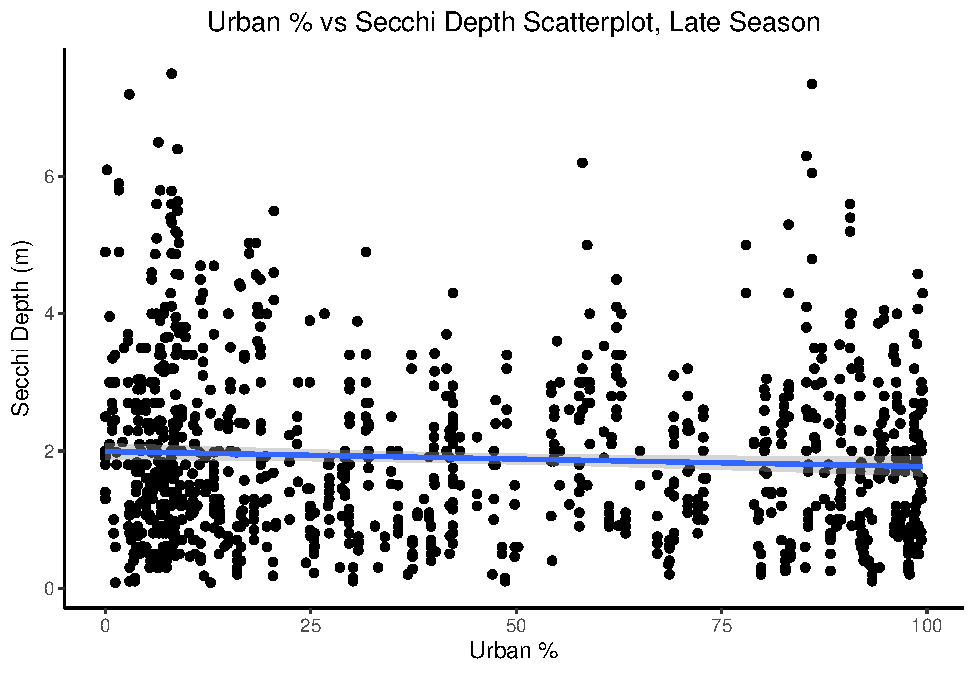
\includegraphics{Bollt_Greif_Raby_Roth_Project_Draft_files/figure-latex/scatterplots-2.pdf}

\begin{Shaded}
\begin{Highlighting}[]
\KeywordTok{ggplot}\NormalTok{(LAGOS.MN.processed.Late.sf, }\KeywordTok{aes}\NormalTok{(}\DataTypeTok{x =}\NormalTok{ Ag.pct, }\DataTypeTok{y =}\NormalTok{ secchi)) }\OperatorTok{+}
\KeywordTok{geom_point}\NormalTok{() }\OperatorTok{+}
\KeywordTok{geom_smooth}\NormalTok{(}\DataTypeTok{method=}\NormalTok{lm) }\OperatorTok{+}
\KeywordTok{xlab}\NormalTok{(}\KeywordTok{expression}\NormalTok{(}\StringTok{"Agriculture %"}\NormalTok{)) }\OperatorTok{+}
\KeywordTok{ylab}\NormalTok{(}\KeywordTok{expression}\NormalTok{(}\StringTok{"Secchi Depth (m)"}\NormalTok{)) }\OperatorTok{+}
\KeywordTok{ggtitle}\NormalTok{(}\StringTok{"Agriculture % vs Secchi Depth Scatterplot, Late Season"}\NormalTok{) }\OperatorTok{+}
\KeywordTok{theme}\NormalTok{(}\DataTypeTok{plot.title =} \KeywordTok{element_text}\NormalTok{(}\DataTypeTok{hjust =} \FloatTok{0.5}\NormalTok{))}
\end{Highlighting}
\end{Shaded}

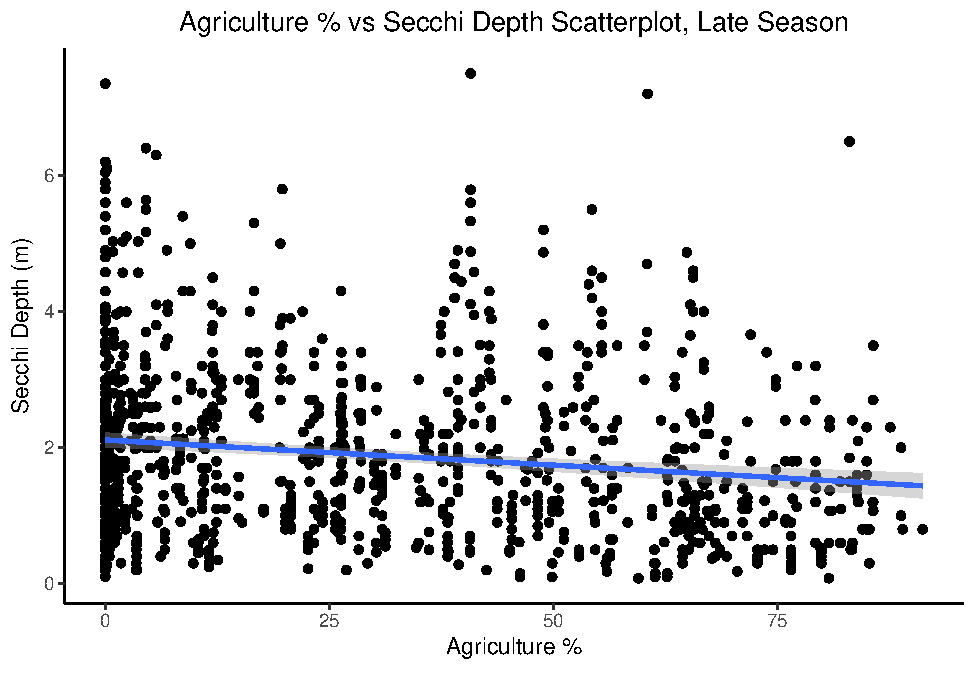
\includegraphics{Bollt_Greif_Raby_Roth_Project_Draft_files/figure-latex/scatterplots-3.pdf}

\begin{Shaded}
\begin{Highlighting}[]
\KeywordTok{ggplot}\NormalTok{(LAGOS.MN.processed.Late.sf, }\KeywordTok{aes}\NormalTok{(}\DataTypeTok{x =}\NormalTok{ Undeveloped.pct, }\DataTypeTok{y =}\NormalTok{ chla)) }\OperatorTok{+}
\KeywordTok{geom_point}\NormalTok{() }\OperatorTok{+}
\KeywordTok{geom_smooth}\NormalTok{(}\DataTypeTok{method=}\NormalTok{lm) }\OperatorTok{+}
\KeywordTok{xlab}\NormalTok{(}\KeywordTok{expression}\NormalTok{(}\StringTok{"Undeveloped %"}\NormalTok{)) }\OperatorTok{+}
\KeywordTok{ylab}\NormalTok{(}\KeywordTok{expression}\NormalTok{(}\StringTok{"Chla (mg/L)"}\NormalTok{)) }\OperatorTok{+}
\KeywordTok{ggtitle}\NormalTok{(}\StringTok{"Undeveloped % vs Chla Scatterplot, Late Season"}\NormalTok{) }\OperatorTok{+}
\KeywordTok{theme}\NormalTok{(}\DataTypeTok{plot.title =} \KeywordTok{element_text}\NormalTok{(}\DataTypeTok{hjust =} \FloatTok{0.5}\NormalTok{))}
\end{Highlighting}
\end{Shaded}

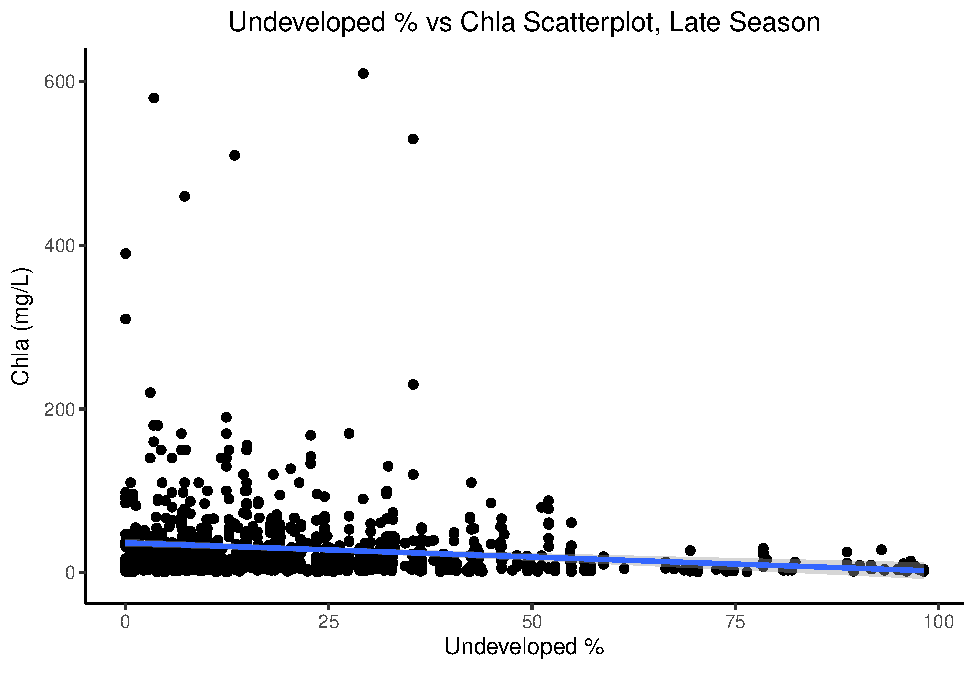
\includegraphics{Bollt_Greif_Raby_Roth_Project_Draft_files/figure-latex/scatterplots-4.pdf}

\begin{Shaded}
\begin{Highlighting}[]
\KeywordTok{ggplot}\NormalTok{(LAGOS.MN.processed.Late.sf, }\KeywordTok{aes}\NormalTok{(}\DataTypeTok{x =}\NormalTok{ Urban.pct, }\DataTypeTok{y =}\NormalTok{ chla)) }\OperatorTok{+}
\KeywordTok{geom_point}\NormalTok{() }\OperatorTok{+}
\KeywordTok{geom_smooth}\NormalTok{(}\DataTypeTok{method=}\NormalTok{lm) }\OperatorTok{+}
\KeywordTok{xlab}\NormalTok{(}\KeywordTok{expression}\NormalTok{(}\StringTok{"Urban %"}\NormalTok{)) }\OperatorTok{+}
\KeywordTok{ylab}\NormalTok{(}\KeywordTok{expression}\NormalTok{(}\StringTok{"Chla (mg/L)"}\NormalTok{)) }\OperatorTok{+}
\KeywordTok{ggtitle}\NormalTok{(}\StringTok{"Urban % vs Chla Scatterplot, Late Season"}\NormalTok{) }\OperatorTok{+}
\KeywordTok{theme}\NormalTok{(}\DataTypeTok{plot.title =} \KeywordTok{element_text}\NormalTok{(}\DataTypeTok{hjust =} \FloatTok{0.5}\NormalTok{))}
\end{Highlighting}
\end{Shaded}

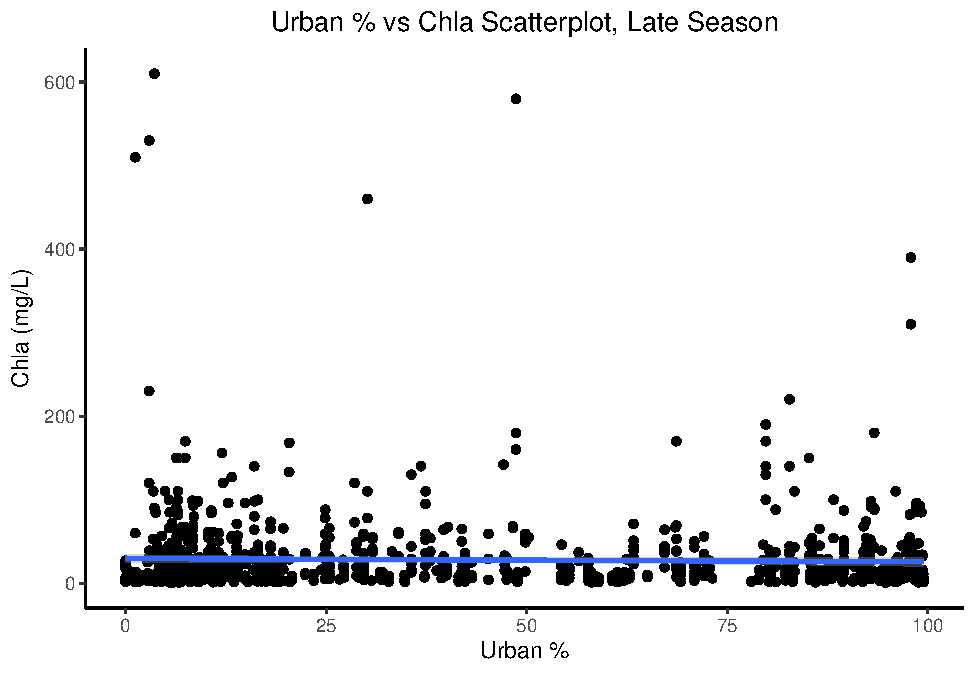
\includegraphics{Bollt_Greif_Raby_Roth_Project_Draft_files/figure-latex/scatterplots-5.pdf}

\begin{Shaded}
\begin{Highlighting}[]
\KeywordTok{ggplot}\NormalTok{(LAGOS.MN.processed.Late.sf, }\KeywordTok{aes}\NormalTok{(}\DataTypeTok{x =}\NormalTok{ Ag.pct, }\DataTypeTok{y =}\NormalTok{ chla)) }\OperatorTok{+}
\KeywordTok{geom_point}\NormalTok{() }\OperatorTok{+}
\KeywordTok{geom_smooth}\NormalTok{(}\DataTypeTok{method=}\NormalTok{lm) }\OperatorTok{+}
\KeywordTok{xlab}\NormalTok{(}\KeywordTok{expression}\NormalTok{(}\StringTok{"Agriculture %"}\NormalTok{)) }\OperatorTok{+}
\KeywordTok{ylab}\NormalTok{(}\KeywordTok{expression}\NormalTok{(}\StringTok{"Chla (mg/L)"}\NormalTok{)) }\OperatorTok{+}
\KeywordTok{ggtitle}\NormalTok{(}\StringTok{"Agriculture % vs Chla Scatterplot, Late Season"}\NormalTok{) }\OperatorTok{+}
\KeywordTok{theme}\NormalTok{(}\DataTypeTok{plot.title =} \KeywordTok{element_text}\NormalTok{(}\DataTypeTok{hjust =} \FloatTok{0.5}\NormalTok{))}
\end{Highlighting}
\end{Shaded}

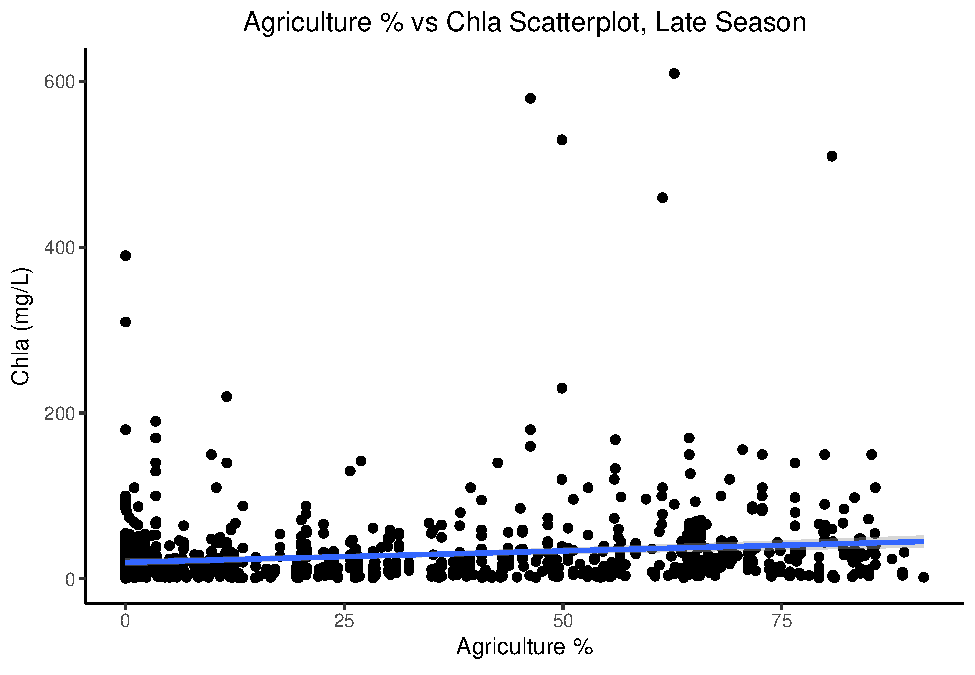
\includegraphics{Bollt_Greif_Raby_Roth_Project_Draft_files/figure-latex/scatterplots-6.pdf}

Late season has the highest mean Chla concentrations and lowest Secchi
depth, so next we explore spatially the variables only for this season
(to minimize maps output).

\begin{Shaded}
\begin{Highlighting}[]
\NormalTok{LAGOS.MN.Summary.Late <-}\StringTok{ }\NormalTok{LAGOS.MN.processed.Late }\OperatorTok
\KeywordTok{group_by}\NormalTok{(lagoslakeid) }\OperatorTok
\KeywordTok{summarise}\NormalTok{(}\DataTypeTok{secchi.mean =} \KeywordTok{mean}\NormalTok{(secchi),}
          \DataTypeTok{chla.mean =} \KeywordTok{mean}\NormalTok{(chla),}
          \DataTypeTok{lake.area =} \KeywordTok{mean}\NormalTok{(lake_area_ha),}
          \DataTypeTok{iws.area =} \KeywordTok{mean}\NormalTok{(iws_ha),}
          \DataTypeTok{LakeIWS.Ratio =} \KeywordTok{mean}\NormalTok{(LakeIWS.Ratio),}
          \DataTypeTok{Water.pct =} \KeywordTok{mean}\NormalTok{(Water.pct),}
          \DataTypeTok{Urban.pct =} \KeywordTok{mean}\NormalTok{(Urban.pct),}
          \DataTypeTok{Undeveloped.pct =} \KeywordTok{mean}\NormalTok{(Undeveloped.pct),}
          \DataTypeTok{Ag.pct =} \KeywordTok{mean}\NormalTok{(Ag.pct),}
          \DataTypeTok{Lat =} \KeywordTok{mean}\NormalTok{(nhd_lat),}
          \DataTypeTok{Long =} \KeywordTok{mean}\NormalTok{(nhd_long)}
\NormalTok{          ) }\OperatorTok
\StringTok{  }\KeywordTok{drop_na}\NormalTok{()}

\CommentTok{#SF file with the summary}
\NormalTok{LAGOS.MN.Summary.Late.sf <-}\StringTok{ }\KeywordTok{st_as_sf}\NormalTok{(LAGOS.MN.Summary.Late, }
                                     \DataTypeTok{coords =} \KeywordTok{c}\NormalTok{(}\StringTok{"Long"}\NormalTok{, }\StringTok{"Lat"}\NormalTok{), }\DataTypeTok{crs =} \DecValTok{4326}\NormalTok{)}

\CommentTok{#Loading the MN state boundary  }
\CommentTok{# generate a map of U.S. states}
\NormalTok{states <-}\StringTok{ }\KeywordTok{st_as_sf}\NormalTok{(}\KeywordTok{map}\NormalTok{(}\DataTypeTok{database =} \StringTok{"state"}\NormalTok{, }\DataTypeTok{plot =} \OtherTok{FALSE}\NormalTok{, }
                       \DataTypeTok{fill =} \OtherTok{TRUE}\NormalTok{, }\DataTypeTok{col =} \StringTok{"white"}\NormalTok{))}

\CommentTok{# filter MN}
\NormalTok{states.MN <-}\StringTok{ }\KeywordTok{filter}\NormalTok{(states, ID }\OperatorTok
\KeywordTok{c}\NormalTok{(}\StringTok{"minnesota"}\NormalTok{))}

\NormalTok{secchiplot1.Late.MN <-}\StringTok{ }\KeywordTok{ggplot}\NormalTok{() }\OperatorTok{+}
\StringTok{  }\KeywordTok{geom_sf}\NormalTok{(}\DataTypeTok{data =}\NormalTok{ states.MN, }\DataTypeTok{fill =} \StringTok{"white"}\NormalTok{) }\OperatorTok{+}
\StringTok{  }\KeywordTok{geom_sf}\NormalTok{(}\DataTypeTok{data =}\NormalTok{ LAGOS.MN.Summary.Late.sf, }
          \KeywordTok{aes}\NormalTok{(}\DataTypeTok{size =}\NormalTok{ Undeveloped.pct, }\DataTypeTok{color =}\NormalTok{ secchi.mean),}
          \DataTypeTok{alpha =} \FloatTok{0.4}\NormalTok{, }\DataTypeTok{show.legend =} \StringTok{"point"}\NormalTok{) }\OperatorTok{+}
\StringTok{  }\KeywordTok{scale_color_viridis_c}\NormalTok{(}\DataTypeTok{option =} \StringTok{"inferno"}\NormalTok{) }\OperatorTok{+}
\StringTok{  }\KeywordTok{labs}\NormalTok{(}\DataTypeTok{color =} \StringTok{"Average }\CharTok{\textbackslash{}n}\StringTok{ Secchi }\CharTok{\textbackslash{}n}\StringTok{ Depth (m)"}\NormalTok{, }
       \DataTypeTok{size =} \StringTok{"Undeveloped }\CharTok{\textbackslash{}n}\StringTok{ Area }\CharTok{\textbackslash{}n}\StringTok{ %"}\NormalTok{) }\OperatorTok{+}
\StringTok{  }\KeywordTok{theme}\NormalTok{(}\DataTypeTok{legend.position =} \StringTok{"right"}\NormalTok{, }\DataTypeTok{legend.text =} \KeywordTok{element_text}\NormalTok{(}\DataTypeTok{size =} \DecValTok{7}\NormalTok{),}
        \DataTypeTok{legend.title =} \KeywordTok{element_text}\NormalTok{(}\DataTypeTok{size =} \DecValTok{8}\NormalTok{),}
        \DataTypeTok{legend.margin =} \KeywordTok{margin}\NormalTok{(}\DecValTok{0}\NormalTok{,}\DecValTok{0}\NormalTok{,}\DecValTok{0}\NormalTok{,}\DecValTok{0}\NormalTok{)) }
\KeywordTok{print}\NormalTok{(secchiplot1.Late.MN)}
\end{Highlighting}
\end{Shaded}

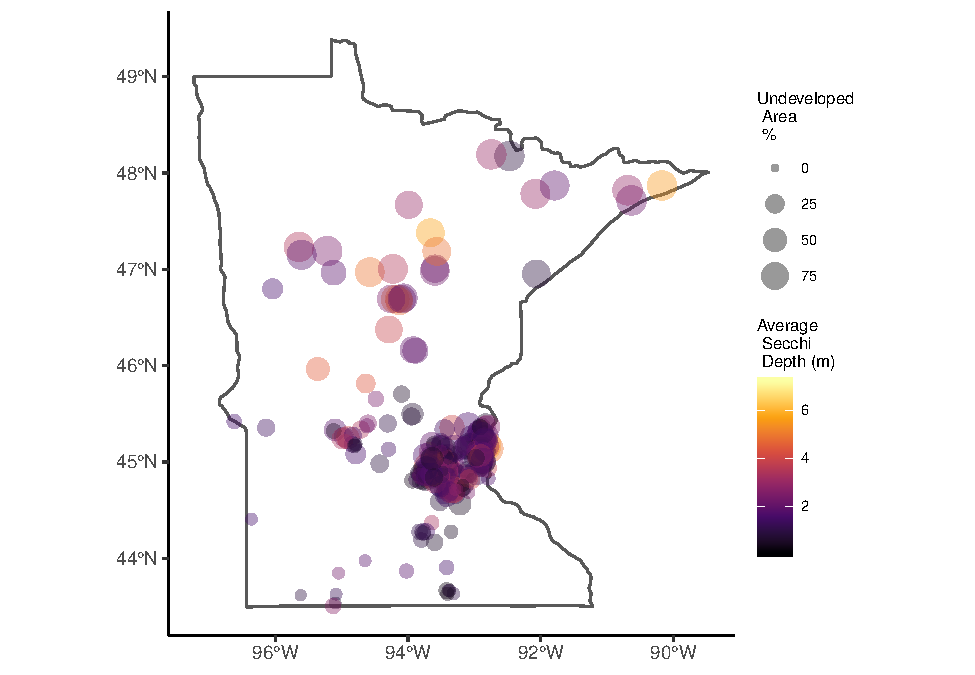
\includegraphics{Bollt_Greif_Raby_Roth_Project_Draft_files/figure-latex/summary.for.late.season-1.pdf}

\begin{Shaded}
\begin{Highlighting}[]
\NormalTok{secchiplot2.Late.MN <-}\StringTok{ }\KeywordTok{ggplot}\NormalTok{() }\OperatorTok{+}
\StringTok{  }\KeywordTok{geom_sf}\NormalTok{(}\DataTypeTok{data =}\NormalTok{ states.MN, }\DataTypeTok{fill =} \StringTok{"white"}\NormalTok{) }\OperatorTok{+}
\StringTok{  }\KeywordTok{geom_sf}\NormalTok{(}\DataTypeTok{data =}\NormalTok{ LAGOS.MN.Summary.Late.sf, }
          \KeywordTok{aes}\NormalTok{(}\DataTypeTok{size =}\NormalTok{ Urban.pct, }\DataTypeTok{color =}\NormalTok{ secchi.mean),}
          \DataTypeTok{alpha =} \FloatTok{0.4}\NormalTok{, }\DataTypeTok{show.legend =} \StringTok{"point"}\NormalTok{) }\OperatorTok{+}
\StringTok{  }\KeywordTok{scale_color_viridis_c}\NormalTok{(}\DataTypeTok{option =} \StringTok{"inferno"}\NormalTok{) }\OperatorTok{+}
\StringTok{  }\KeywordTok{labs}\NormalTok{(}\DataTypeTok{color =} \StringTok{"Average }\CharTok{\textbackslash{}n}\StringTok{ Secchi }\CharTok{\textbackslash{}n}\StringTok{ Depth (m)"}\NormalTok{, }
       \DataTypeTok{size =} \StringTok{"Urban }\CharTok{\textbackslash{}n}\StringTok{ Area }\CharTok{\textbackslash{}n}\StringTok{ %"}\NormalTok{) }\OperatorTok{+}
\StringTok{  }\KeywordTok{theme}\NormalTok{(}\DataTypeTok{legend.position =} \StringTok{"right"}\NormalTok{, }\DataTypeTok{legend.text =} \KeywordTok{element_text}\NormalTok{(}\DataTypeTok{size =} \DecValTok{7}\NormalTok{),}
        \DataTypeTok{legend.title =} \KeywordTok{element_text}\NormalTok{(}\DataTypeTok{size =} \DecValTok{8}\NormalTok{),}
        \DataTypeTok{legend.margin =} \KeywordTok{margin}\NormalTok{(}\DecValTok{0}\NormalTok{,}\DecValTok{0}\NormalTok{,}\DecValTok{0}\NormalTok{,}\DecValTok{0}\NormalTok{)) }
\KeywordTok{print}\NormalTok{(secchiplot2.Late.MN)}
\end{Highlighting}
\end{Shaded}

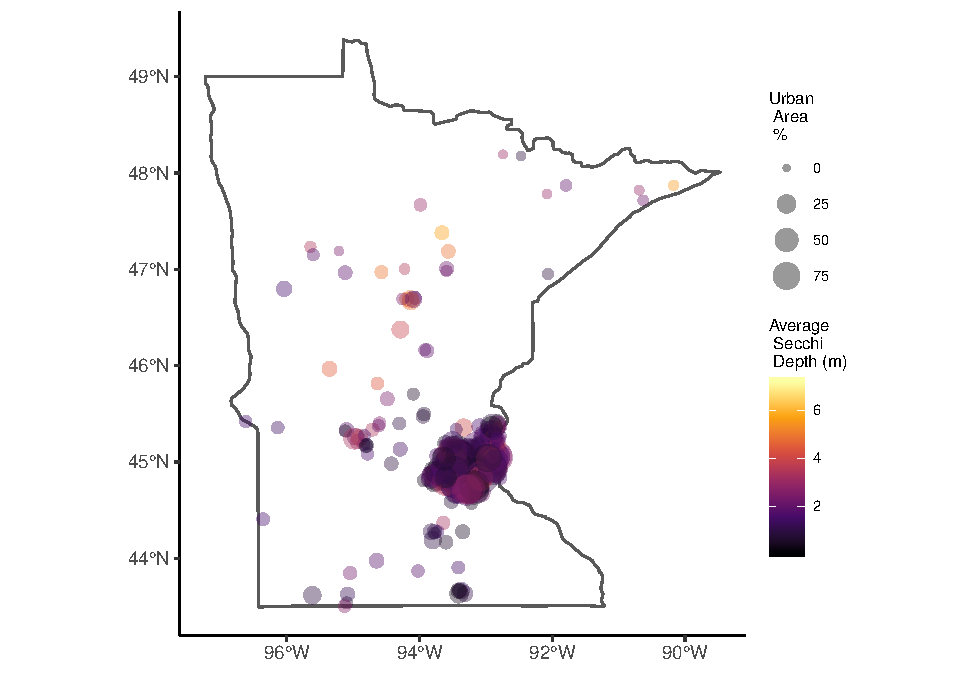
\includegraphics{Bollt_Greif_Raby_Roth_Project_Draft_files/figure-latex/summary.for.late.season-2.pdf}

\begin{Shaded}
\begin{Highlighting}[]
\NormalTok{secchiplot3.Late.MN <-}\StringTok{ }\KeywordTok{ggplot}\NormalTok{() }\OperatorTok{+}
\StringTok{  }\KeywordTok{geom_sf}\NormalTok{(}\DataTypeTok{data =}\NormalTok{ states.MN, }\DataTypeTok{fill =} \StringTok{"white"}\NormalTok{) }\OperatorTok{+}
\StringTok{  }\KeywordTok{geom_sf}\NormalTok{(}\DataTypeTok{data =}\NormalTok{ LAGOS.MN.Summary.Late.sf, }
          \KeywordTok{aes}\NormalTok{(}\DataTypeTok{size =}\NormalTok{ Ag.pct, }\DataTypeTok{color =}\NormalTok{ secchi.mean),}
          \DataTypeTok{alpha =} \FloatTok{0.4}\NormalTok{, }\DataTypeTok{show.legend =} \StringTok{"point"}\NormalTok{) }\OperatorTok{+}
\StringTok{  }\KeywordTok{scale_color_viridis_c}\NormalTok{(}\DataTypeTok{option =} \StringTok{"inferno"}\NormalTok{) }\OperatorTok{+}
\StringTok{  }\KeywordTok{labs}\NormalTok{(}\DataTypeTok{color =} \StringTok{"Average }\CharTok{\textbackslash{}n}\StringTok{ Secchi }\CharTok{\textbackslash{}n}\StringTok{ Depth (m)"}\NormalTok{, }
       \DataTypeTok{size =} \StringTok{"Agricultural }\CharTok{\textbackslash{}n}\StringTok{ Area }\CharTok{\textbackslash{}n}\StringTok{ %"}\NormalTok{) }\OperatorTok{+}
\StringTok{  }\KeywordTok{theme}\NormalTok{(}\DataTypeTok{legend.position =} \StringTok{"right"}\NormalTok{, }\DataTypeTok{legend.text =} \KeywordTok{element_text}\NormalTok{(}\DataTypeTok{size =} \DecValTok{7}\NormalTok{),}
        \DataTypeTok{legend.title =} \KeywordTok{element_text}\NormalTok{(}\DataTypeTok{size =} \DecValTok{8}\NormalTok{),}
        \DataTypeTok{legend.margin =} \KeywordTok{margin}\NormalTok{(}\DecValTok{0}\NormalTok{,}\DecValTok{0}\NormalTok{,}\DecValTok{0}\NormalTok{,}\DecValTok{0}\NormalTok{)) }
\KeywordTok{print}\NormalTok{(secchiplot3.Late.MN)}
\end{Highlighting}
\end{Shaded}

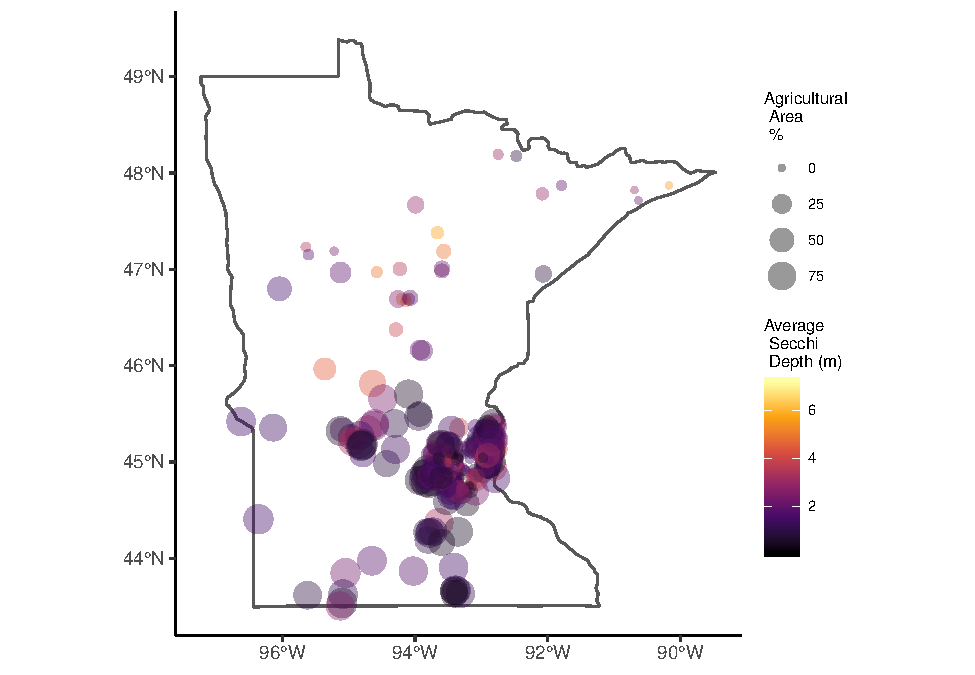
\includegraphics{Bollt_Greif_Raby_Roth_Project_Draft_files/figure-latex/summary.for.late.season-3.pdf}

\begin{Shaded}
\begin{Highlighting}[]
\NormalTok{chlaplot1.Late.MN <-}\StringTok{ }\KeywordTok{ggplot}\NormalTok{() }\OperatorTok{+}
\StringTok{  }\KeywordTok{geom_sf}\NormalTok{(}\DataTypeTok{data =}\NormalTok{ states.MN, }\DataTypeTok{fill =} \StringTok{"white"}\NormalTok{) }\OperatorTok{+}
\StringTok{  }\KeywordTok{geom_sf}\NormalTok{(}\DataTypeTok{data =}\NormalTok{ LAGOS.MN.Summary.Late.sf, }
          \KeywordTok{aes}\NormalTok{(}\DataTypeTok{size =}\NormalTok{ Undeveloped.pct, }\DataTypeTok{color =}\NormalTok{ chla.mean),}
          \DataTypeTok{alpha =} \FloatTok{0.4}\NormalTok{, }\DataTypeTok{show.legend =} \StringTok{"point"}\NormalTok{) }\OperatorTok{+}
\StringTok{  }\KeywordTok{scale_color_viridis_c}\NormalTok{(}\DataTypeTok{option =} \StringTok{"inferno"}\NormalTok{) }\OperatorTok{+}
\StringTok{  }\KeywordTok{labs}\NormalTok{(}\DataTypeTok{color =} \StringTok{"Average }\CharTok{\textbackslash{}n}\StringTok{ Chla }\CharTok{\textbackslash{}n}\StringTok{ Depth (m)"}\NormalTok{, }
       \DataTypeTok{size =} \StringTok{"Undeveloped }\CharTok{\textbackslash{}n}\StringTok{ Area }\CharTok{\textbackslash{}n}\StringTok{ %"}\NormalTok{) }\OperatorTok{+}
\StringTok{  }\KeywordTok{theme}\NormalTok{(}\DataTypeTok{legend.position =} \StringTok{"right"}\NormalTok{, }\DataTypeTok{legend.text =} \KeywordTok{element_text}\NormalTok{(}\DataTypeTok{size =} \DecValTok{7}\NormalTok{),}
        \DataTypeTok{legend.title =} \KeywordTok{element_text}\NormalTok{(}\DataTypeTok{size =} \DecValTok{8}\NormalTok{),}
        \DataTypeTok{legend.margin =} \KeywordTok{margin}\NormalTok{(}\DecValTok{0}\NormalTok{,}\DecValTok{0}\NormalTok{,}\DecValTok{0}\NormalTok{,}\DecValTok{0}\NormalTok{)) }
\KeywordTok{print}\NormalTok{(chlaplot1.Late.MN)}
\end{Highlighting}
\end{Shaded}

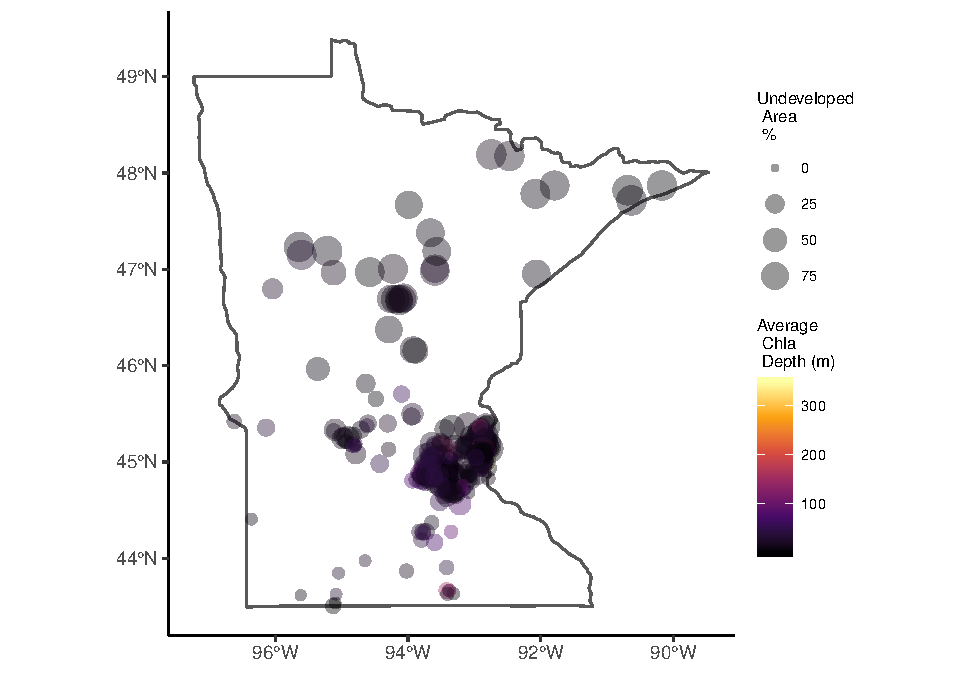
\includegraphics{Bollt_Greif_Raby_Roth_Project_Draft_files/figure-latex/summary.for.late.season-4.pdf}

\begin{Shaded}
\begin{Highlighting}[]
\NormalTok{chlaplot2.Late.MN <-}\StringTok{ }\KeywordTok{ggplot}\NormalTok{() }\OperatorTok{+}
\StringTok{  }\KeywordTok{geom_sf}\NormalTok{(}\DataTypeTok{data =}\NormalTok{ states.MN, }\DataTypeTok{fill =} \StringTok{"white"}\NormalTok{) }\OperatorTok{+}
\StringTok{  }\KeywordTok{geom_sf}\NormalTok{(}\DataTypeTok{data =}\NormalTok{ LAGOS.MN.Summary.Late.sf, }
          \KeywordTok{aes}\NormalTok{(}\DataTypeTok{size =}\NormalTok{ Urban.pct, }\DataTypeTok{color =}\NormalTok{ chla.mean),}
          \DataTypeTok{alpha =} \FloatTok{0.4}\NormalTok{, }\DataTypeTok{show.legend =} \StringTok{"point"}\NormalTok{) }\OperatorTok{+}
\StringTok{  }\KeywordTok{scale_color_viridis_c}\NormalTok{(}\DataTypeTok{option =} \StringTok{"inferno"}\NormalTok{) }\OperatorTok{+}
\StringTok{  }\KeywordTok{labs}\NormalTok{(}\DataTypeTok{color =} \StringTok{"Average }\CharTok{\textbackslash{}n}\StringTok{ Chla }\CharTok{\textbackslash{}n}\StringTok{ Depth (m)"}\NormalTok{, }
       \DataTypeTok{size =} \StringTok{"Urban }\CharTok{\textbackslash{}n}\StringTok{ Area }\CharTok{\textbackslash{}n}\StringTok{ %"}\NormalTok{) }\OperatorTok{+}
\StringTok{  }\KeywordTok{theme}\NormalTok{(}\DataTypeTok{legend.position =} \StringTok{"right"}\NormalTok{, }\DataTypeTok{legend.text =} \KeywordTok{element_text}\NormalTok{(}\DataTypeTok{size =} \DecValTok{7}\NormalTok{),}
        \DataTypeTok{legend.title =} \KeywordTok{element_text}\NormalTok{(}\DataTypeTok{size =} \DecValTok{8}\NormalTok{),}
        \DataTypeTok{legend.margin =} \KeywordTok{margin}\NormalTok{(}\DecValTok{0}\NormalTok{,}\DecValTok{0}\NormalTok{,}\DecValTok{0}\NormalTok{,}\DecValTok{0}\NormalTok{)) }
\KeywordTok{print}\NormalTok{(chlaplot2.Late.MN)}
\end{Highlighting}
\end{Shaded}

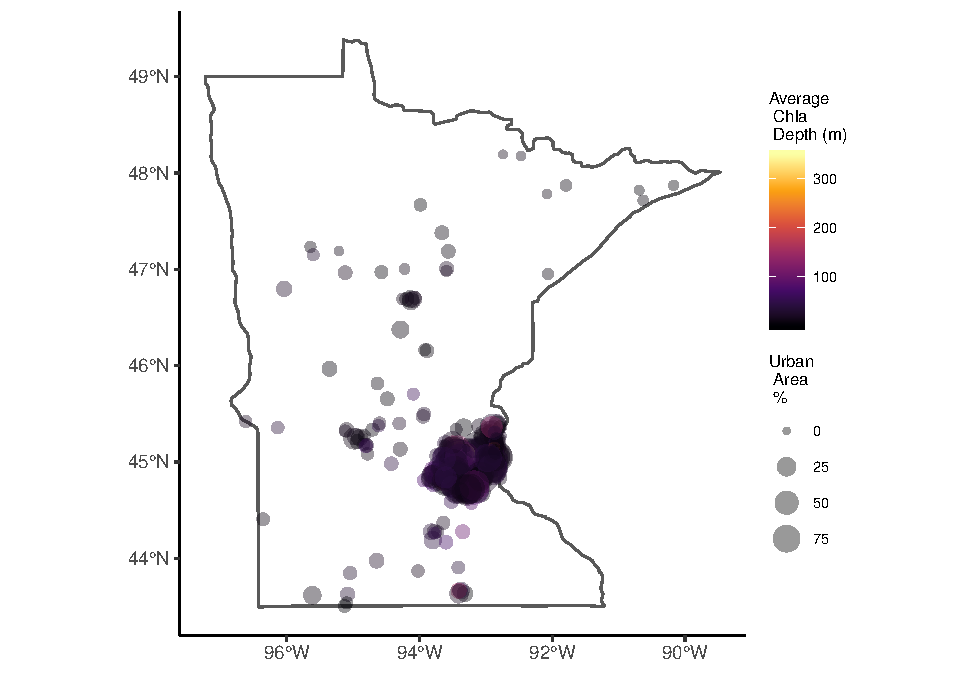
\includegraphics{Bollt_Greif_Raby_Roth_Project_Draft_files/figure-latex/summary.for.late.season-5.pdf}

\begin{Shaded}
\begin{Highlighting}[]
\NormalTok{chlaplot3.Late.MN <-}\StringTok{ }\KeywordTok{ggplot}\NormalTok{() }\OperatorTok{+}
\StringTok{  }\KeywordTok{geom_sf}\NormalTok{(}\DataTypeTok{data =}\NormalTok{ states.MN, }\DataTypeTok{fill =} \StringTok{"white"}\NormalTok{) }\OperatorTok{+}
\StringTok{  }\KeywordTok{geom_sf}\NormalTok{(}\DataTypeTok{data =}\NormalTok{ LAGOS.MN.Summary.Late.sf, }
          \KeywordTok{aes}\NormalTok{(}\DataTypeTok{size =}\NormalTok{ Ag.pct, }\DataTypeTok{color =}\NormalTok{ chla.mean),}
          \DataTypeTok{alpha =} \FloatTok{0.4}\NormalTok{, }\DataTypeTok{show.legend =} \StringTok{"point"}\NormalTok{) }\OperatorTok{+}
\StringTok{  }\KeywordTok{scale_color_viridis_c}\NormalTok{(}\DataTypeTok{option =} \StringTok{"inferno"}\NormalTok{) }\OperatorTok{+}
\StringTok{  }\KeywordTok{labs}\NormalTok{(}\DataTypeTok{color =} \StringTok{"Average }\CharTok{\textbackslash{}n}\StringTok{ Chla }\CharTok{\textbackslash{}n}\StringTok{ Depth (m)"}\NormalTok{, }
       \DataTypeTok{size =} \StringTok{"Agricultural }\CharTok{\textbackslash{}n}\StringTok{ Area }\CharTok{\textbackslash{}n}\StringTok{ %"}\NormalTok{) }\OperatorTok{+}
\StringTok{  }\KeywordTok{theme}\NormalTok{(}\DataTypeTok{legend.position =} \StringTok{"right"}\NormalTok{, }\DataTypeTok{legend.text =} \KeywordTok{element_text}\NormalTok{(}\DataTypeTok{size =} \DecValTok{7}\NormalTok{),}
        \DataTypeTok{legend.title =} \KeywordTok{element_text}\NormalTok{(}\DataTypeTok{size =} \DecValTok{8}\NormalTok{),}
        \DataTypeTok{legend.margin =} \KeywordTok{margin}\NormalTok{(}\DecValTok{0}\NormalTok{,}\DecValTok{0}\NormalTok{,}\DecValTok{0}\NormalTok{,}\DecValTok{0}\NormalTok{)) }
\KeywordTok{print}\NormalTok{(secchiplot3.Late.MN)}
\end{Highlighting}
\end{Shaded}

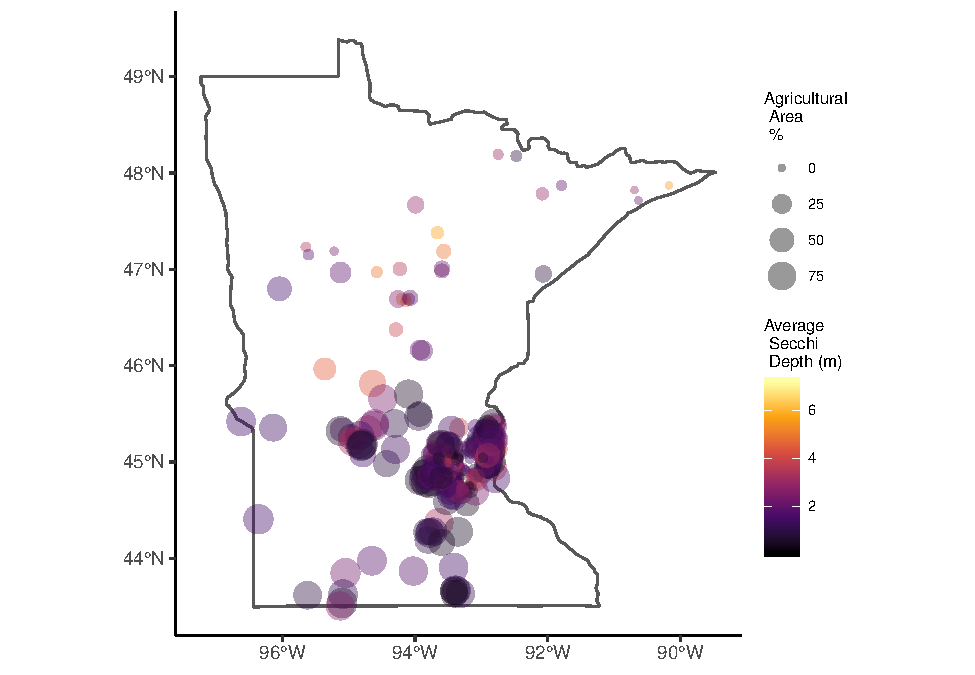
\includegraphics{Bollt_Greif_Raby_Roth_Project_Draft_files/figure-latex/summary.for.late.season-6.pdf}

\begin{Shaded}
\begin{Highlighting}[]
\KeywordTok{st_geometry}\NormalTok{(LAGOS.MN.processed.Early.sf) <-}\StringTok{ }\OtherTok{NULL}
\KeywordTok{write.csv}\NormalTok{(}\DataTypeTok{x =}\NormalTok{  LAGOS.MN.processed.Early.sf, }\DataTypeTok{row.names =} \OtherTok{FALSE}\NormalTok{,}
          \DataTypeTok{file =}  \StringTok{"./data/processed/LAGOS.MN.processed.Early.csv"}\NormalTok{)}

\KeywordTok{st_geometry}\NormalTok{(LAGOS.MN.processed.Prime.sf) <-}\StringTok{ }\OtherTok{NULL}
\KeywordTok{write.csv}\NormalTok{(}\DataTypeTok{x =}\NormalTok{  LAGOS.MN.processed.Prime.sf, }\DataTypeTok{row.names =} \OtherTok{FALSE}\NormalTok{,}
          \DataTypeTok{file =}  \StringTok{"./data/processed/LAGOS.MN.processed.Prime.csv"}\NormalTok{)}

\KeywordTok{st_geometry}\NormalTok{(LAGOS.MN.processed.Late.sf) <-}\StringTok{ }\OtherTok{NULL}
\KeywordTok{write.csv}\NormalTok{(}\DataTypeTok{x =}\NormalTok{  LAGOS.MN.processed.Late.sf, }\DataTypeTok{row.names =} \OtherTok{FALSE}\NormalTok{,}
          \DataTypeTok{file =}  \StringTok{"./data/processed/LAGOS.MN.processed.Late.csv"}\NormalTok{)}
\end{Highlighting}
\end{Shaded}

\newpage

\hypertarget{analysis}{%
\section{Analysis}\label{analysis}}

\begin{itemize}
\tightlist
\item
  First we will create correlation plots in order to eliminate variables
  with a correlation greater than 0.8.
\item
  Then we will run Shapiro-Wilkes tests to determine normality and the
  need for possible data transformations.
\item
  After determining the distributions of the data, we will generate
  mixed effect linear models with chlorophyll a and secchi depth as
  response variables, land use and lake-watershed area ratio as fixed
  effects, and ecoregion as a random effect.
\end{itemize}

Final figures will include:

\begin{itemize}
\tightlist
\item
  6 maps of the state, each showing the relationship between land use
  and both response variables. Ecoregion will be included as a base
  layer for each map.
\item
  Scatter plots showing the strongest relationships between land use and
  the response variables.
\item
  Table showing results of linear model.
\end{itemize}

\newpage

\hypertarget{summary-and-conclusions}{%
\section{Summary and Conclusions}\label{summary-and-conclusions}}

\begin{itemize}
\tightlist
\item
  Conclusions will include a discussion of our results within the
  context of MN nutrient management plan.
\end{itemize}


\end{document}
